% Generated by `uv run analyze`; needs \usepackage{pgfplots}
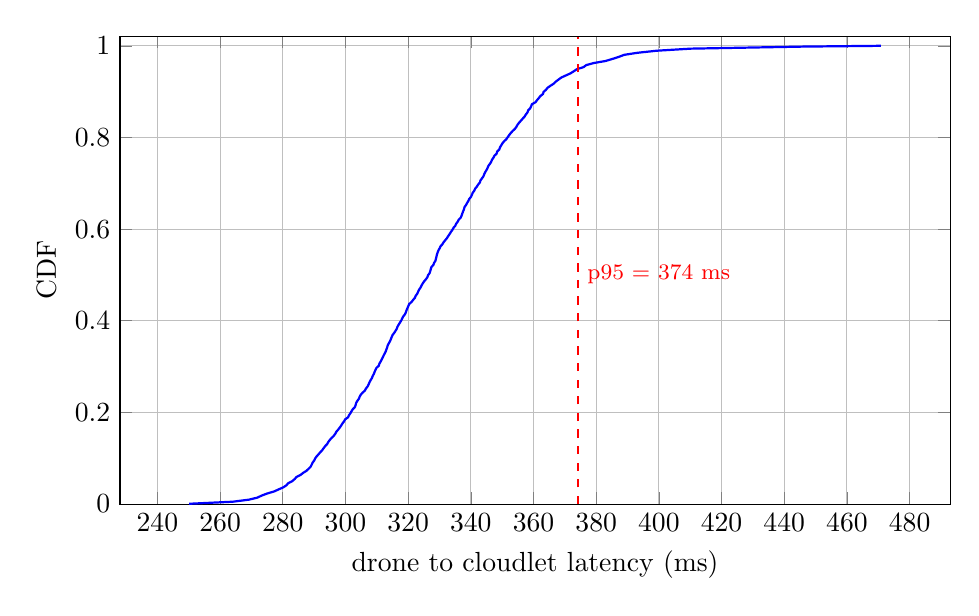
\begin{tikzpicture}
\begin{axis}[xlabel={drone to cloudlet latency (ms)}, ylabel={CDF}, width=\columnwidth, height=0.62\columnwidth, grid=major, ymin=0, ymax=1.02]
\addplot[thick, blue] coordinates {(250.126,0.0006) (264.037,0.0051) (269.226,0.0096) (271.878,0.0140) (273.279,0.0185) (275.013,0.0230) (277.226,0.0275) (278.686,0.0320) (280.177,0.0365) (281.183,0.0410) (281.706,0.0455) (283.022,0.0500) (283.792,0.0545) (284.368,0.0590) (285.651,0.0635) (286.492,0.0680) (287.555,0.0725) (288.231,0.0770) (288.893,0.0815) (289.226,0.0860) (289.531,0.0904) (290.005,0.0949) (290.325,0.0994) (290.793,0.1039) (291.379,0.1084) (291.956,0.1129) (292.566,0.1174) (293.04,0.1219) (293.53,0.1264) (294.163,0.1309) (294.526,0.1354) (295.006,0.1399) (295.598,0.1444) (296.286,0.1489) (296.748,0.1534) (297.107,0.1579) (297.681,0.1624) (298.188,0.1669) (298.627,0.1713) (299.03,0.1758) (299.537,0.1803) (299.895,0.1848) (300.826,0.1893) (301.124,0.1938) (301.594,0.1983) (301.955,0.2028) (302.39,0.2073) (303.023,0.2118) (303.258,0.2163) (303.419,0.2208) (303.808,0.2253) (304.293,0.2298) (304.526,0.2343) (304.905,0.2388) (305.505,0.2433) (306.222,0.2478) (306.535,0.2522) (307.085,0.2567) (307.392,0.2612) (307.666,0.2657) (308.007,0.2702) (308.428,0.2747) (308.684,0.2792) (309.024,0.2837) (309.291,0.2882) (309.57,0.2927) (309.888,0.2972) (310.63,0.3017) (310.813,0.3062) (311.204,0.3107) (311.557,0.3152) (311.882,0.3197) (312.175,0.3242) (312.519,0.3287) (312.863,0.3331) (313.08,0.3376) (313.321,0.3421) (313.498,0.3466) (313.862,0.3511) (314.223,0.3556) (314.508,0.3601) (314.764,0.3646) (315.045,0.3691) (315.565,0.3736) (315.979,0.3781) (316.384,0.3826) (316.61,0.3871) (316.987,0.3916) (317.4,0.3961) (317.805,0.4006) (318.124,0.4051) (318.451,0.4096) (318.973,0.4140) (319.286,0.4185) (319.491,0.4230) (319.775,0.4275) (320.06,0.4320) (320.334,0.4365) (321.082,0.4410) (321.582,0.4455) (322.15,0.4500) (322.412,0.4545) (322.896,0.4590) (323.194,0.4635) (323.52,0.4680) (323.964,0.4725) (324.272,0.4770) (324.664,0.4815) (325.118,0.4860) (325.65,0.4904) (326.138,0.4949) (326.364,0.4994) (326.846,0.5039) (327.068,0.5084) (327.237,0.5129) (327.452,0.5174) (328.054,0.5219) (328.293,0.5264) (328.705,0.5309) (328.878,0.5354) (329.033,0.5399) (329.173,0.5444) (329.416,0.5489) (329.644,0.5534) (330.034,0.5579) (330.325,0.5624) (330.922,0.5669) (331.31,0.5713) (331.847,0.5758) (332.376,0.5803) (332.787,0.5848) (333.248,0.5893) (333.645,0.5938) (334.119,0.5983) (334.471,0.6028) (335.043,0.6073) (335.327,0.6118) (335.82,0.6163) (336.172,0.6208) (336.8,0.6253) (337.07,0.6298) (337.3,0.6343) (337.535,0.6388) (337.819,0.6433) (337.97,0.6478) (338.427,0.6522) (338.788,0.6567) (339.182,0.6612) (339.487,0.6657) (340.032,0.6702) (340.347,0.6747) (340.597,0.6792) (341.074,0.6837) (341.38,0.6882) (341.918,0.6927) (342.34,0.6972) (342.885,0.7017) (343.081,0.7062) (343.557,0.7107) (344.027,0.7152) (344.274,0.7197) (344.574,0.7242) (344.981,0.7287) (345.314,0.7331) (345.576,0.7376) (346.042,0.7421) (346.485,0.7466) (346.732,0.7511) (347.198,0.7556) (347.526,0.7601) (348.213,0.7646) (348.401,0.7691) (349.073,0.7736) (349.282,0.7781) (349.681,0.7826) (350.075,0.7871) (350.604,0.7916) (351.307,0.7961) (351.771,0.8006) (352.227,0.8051) (352.734,0.8096) (353.324,0.8140) (354.02,0.8185) (354.523,0.8230) (354.881,0.8275) (355.383,0.8320) (355.973,0.8365) (356.538,0.8410) (357.151,0.8455) (357.541,0.8500) (358.062,0.8545) (358.286,0.8590) (358.919,0.8635) (359.242,0.8680) (359.49,0.8725) (360.663,0.8770) (361.129,0.8815) (361.698,0.8860) (362.2,0.8904) (363.025,0.8949) (363.211,0.8994) (363.974,0.9039) (364.482,0.9084) (365.429,0.9129) (366.447,0.9174) (367.119,0.9219) (367.99,0.9264) (368.901,0.9309) (370.347,0.9354) (371.795,0.9399) (372.841,0.9444) (373.811,0.9489) (375.945,0.9534) (376.826,0.9579) (379.214,0.9624) (383.007,0.9669) (385.152,0.9713) (387.193,0.9758) (388.935,0.9803) (393.176,0.9848) (399.365,0.9893) (410.178,0.9938) (446.184,0.9983) (470.864,1.0000)};
\draw[red, dashed, thick] (axis cs:374.097,0) -- (axis cs:374.097,1.02);
\node[red, anchor=west, font=\footnotesize] at (axis cs:374.097,0.5) {p95 = 374 ms};
\end{axis}
\end{tikzpicture}
